\documentclass[preprint,12pt,authoryear]{elsarticle}
% ---------------------------------------------------------------------------
% SimTwin preprint.  Self-contained: compile with
%     tectonic paper/main.tex
% All packages used are on CTAN; no local .sty files are required.
% ---------------------------------------------------------------------------
\usepackage{amsmath,amssymb}
\usepackage{graphicx}
\usepackage{booktabs}
\usepackage{array}
\usepackage{url}
\usepackage{xurl}
\usepackage[htt]{hyphenat}
\emergencystretch=3em
\tolerance=1200
\usepackage{fontspec}
\usepackage[hidelinks]{hyperref}

\graphicspath{{figures/}}

\newcommand{\smt}{SimTwin}
\journal{Journal of Open Source Research Software}

\begin{document}

\begin{frontmatter}

\title{\smt{}: an open-source reproducible simulator of networked FDM/FFF
printer fleets with digital-twin synchronisation, fault injection and
communication impairment}

\author[a]{Nata~Sulakvelidze\corref{cor1}}
\ead{nata.sulakvelidze@gmail.com}
\cortext[cor1]{Corresponding author.}
\affiliation[a]{organization={Versec LLC / G3D},
                city={Tbilisi},
                country={Georgia}}

\begin{abstract}
Digital-twin research on additive-manufacturing (AM) fleets needs experiments in
which the physical process, the communication channel and the twin's
synchronisation state can all be manipulated and measured independently.
Existing tools cover fragments of this: discrete-event factory simulators ignore
the physics of the print, thermal and process models of a single machine ignore
the network, and networked-control benchmarks have no plant.
We present \smt{}, an open-source Python simulator that couples
(i) a three-node lumped-parameter thermal plant with proportional--integral
heater control, an additive power model and a road-geometry deposition model,
(ii) a finite-state job and health machine per device,
(iii) an explicit message-level transport with latency, jitter, loss,
duplication, per-device disconnection, broker-wide outage, replay queues and
staleness-based discarding, and
(iv) a twin registry that maintains \emph{reported}, \emph{desired},
\emph{configuration} and \emph{connectivity} aspects separately and is written
only by delivered messages.
Faults are injected as \emph{mechanisms} --- multiplicative changes to heater
efficiency, thermal conductance, parasitic heat load, controller gain, extrusion
scale, motor power, sensor bias and sensor noise, plus terminal job
interruption --- never as scripted telemetry labels, so fault signatures emerge
from the dynamics.
A seed-spawning scheme gives bit-level reproducibility: two runs at the same
seed produce byte-identical telemetry (SHA-256 match), and a change of seed
changes it.
We report seven experiments on a single 11-core laptop:
scalability to 1\,000 printers at 88\,643 device-steps\,s$^{-1}$ and a real-time
factor of 88.6;
telemetry throughput from 686 to 70\,363\,msg\,s$^{-1}$ over a 240-fold sampling
sweep;
delivery ratios that track the configured loss rate to within 0.05 percentage
points while 95th-percentile twin staleness grows from 0.99\,s to 6.99\,s;
outage sweeps in which resynchronisations grow from 0 to 324\,942;
and fault separability in which 10 of 11 injected fault families reach
Cohen's $|d|\ge 1.45$ on at least one observable channel, with
bed-heater failure at $|d|=3.68$ on measured power;
and a broker-fidelity study in which the same messages traverse a real
Mosquitto broker, showing that QoS~1 back-pressure holds 95th-percentile twin
staleness at 1.2\,s while fire-and-forget QoS~0 lets it grow 12.6-fold to 15.1\,s.
Together these give a measurable, citable baseline for twin-synchronisation
quality of service and for mechanism-grounded fault-signature separability in
networked AM fleets.
\end{abstract}

\begin{keyword}
digital twin \sep additive manufacturing \sep fused deposition modeling \sep
fleet simulation \sep fault injection \sep industrial IoT \sep MQTT \sep
age of information \sep reproducibility
\end{keyword}

\end{frontmatter}
\section{Introduction}
\label{sec:intro}
\S\ref{sec:related} positions the work, \S\ref{sec:model} gives the model and
\S\ref{sec:architecture} the implementation, \S\ref{sec:determinism} the
reproducibility contract, \S\ref{sec:eval} the seven experiments, and
\S\ref{sec:limitations}--\S\ref{sec:conclusion} what they mean and do not mean.

Fused deposition modelling (FDM/FFF) fleets are becoming a networked,
instrumented production setting: tens to hundreds of machines report telemetry
over MQTT or OPC~UA to a supervisory layer that maintains a digital twin of each
machine \citep{grieves2016dt,tao2019dtii,barricelli2019dt,fuller2020dt}.
The digital-twin literature is explicit that the value of a twin depends on the
\emph{fidelity} of the model, the \emph{freshness} of its state, and the
\emph{fidelity} of the observed data
\citep{tao2017fivelayer,iso23247,iso30173}, and that synchronisation is itself an
engineering problem with a cost \citep{tan2023sync}.

Research on this setting needs an experiment platform in which three things can
be varied and measured \emph{independently}: the physical process, the
communication channel, and the twin's synchronisation state.
The tools that exist each cover one axis and assume the others away.
Discrete-event factory simulators model queues and stations, not nozzle
thermodynamics.
Thermal and process models of a single extruder \citep{fibremul2020} model the
physics in detail, for one machine, over an ideal channel.
Networked-control-system studies model delay, dropout and scheduling
\citep{walsh2002ncs,zhang2001ncs} over an abstract plant.
Age-of-information (AoI) work quantifies freshness of a source
\citep{kaul2012aoi,yates2021aoi} but has no process to be fresh \emph{about}.
AM fault-detection datasets are dominated by images and single-machine
instrumented runs \citep{szydlowski2021dataset}; predictive-maintenance
benchmarks use machine-tool signals without a fleet, a network, or a twin.

This paper contributes \smt{}, a simulator built to close that gap, and the
reproducible evidence base that comes with it.

\subsection*{Contributions}
\begin{enumerate}
  \item \textbf{A layered architecture with a hard information barrier.}
        Device state, twin-reported state, desired state, configuration and
        connectivity are separate objects. The twin registry is written
        \emph{only} by messages the transport delivered, so twin staleness,
        synchronisation delay and resynchronisation counts are consequences of
        the channel model rather than annotations.
  \item \textbf{Mechanism-level fault injection.} Eleven faults across five
        families are expressed as parameter transformations of the plant and
        observation models (Table~\ref{tab:faults}). Fault signatures are
        emergent, which is what makes a separability study meaningful.
  \item \textbf{Explicit delivery semantics.} Latency with a lognormal tail,
        independent loss, duplication, per-device disconnection with exponential
        reconnect backoff and replay queues, broker-wide outage, and
        staleness-based discarding, all applied in the transport, never in the
        device model.
  \item \textbf{Determinism by construction.} A \texttt{SeedPlan} spawns
        independent named NumPy streams, so a run is a pure function of its
        configuration and seed. We verify this by hashing telemetry.
  \item \textbf{Seven experiments with published artifacts} covering
        scalability, telemetry frequency, network impairment, fault
        separability, outage/recovery, reproducibility and broker fidelity, plus
        a dataset package with provenance metadata.
  \item \textbf{A fully verified bibliography}: every journal, volume, issue,
        page range and DOI in this paper was resolved against the Crossref REST
        API; five candidate sources that could not be resolved were dropped
        (Section~\ref{sec:limitations}).
\end{enumerate}

\smt{} is deliberately \emph{not} a high-fidelity FDM physics simulator. It is a
cyber-physical / industrial-IoT research testbed: the physics is the simplest
lumped model that produces the qualitative behaviour the twin has to track, at a
cost that lets a thousand-machine, hour-long scenario run on a laptop in under a
minute.

\section{Related work}
\label{sec:related}

\subsection{Digital twins in manufacturing}
Grieves' twin formulation separates the physical asset, its virtual model and the
connections between them \citep{grieves2014dt,grieves2016dt}.
Tao et al.\ formalise a five-layer architecture and the requirement for
bidirectional coupling \citep{tao2019dtii,tao2017fivelayer}, and survey
twin-driven smart-manufacturing system design \citep{liu2023dtms}.
Standardisation has caught up: ISO 23247 defines a digital-twin framework for
manufacturing \citep{iso23247} and ISO/IEC 30173 defines digital-twin
representations of physical systems \citep{iso30173}.
Surveys map the enabling-technology landscape \citep{fuller2020dt,barricelli2019dt},
the maturity models used to classify twins \citep{uhlenkamp2022maturity}, and the
methodologies by which twins are built \citep{aznar2026dtm}.
Reference architectures for synchronised twin factories are demonstrated in
\citep{kumar2024dtfactory}, and simulation-based twins for discrete material-flow
systems in \citep{schwede2024sbdm}.
The \emph{synchronisation problem} --- how far a twin may diverge from its
physical twin, how that divergence is formulated, and what it costs to close the
gap --- is treated explicitly by \citet{tan2023sync}.
\smt{} is built to make that divergence measurable: it exposes per-twin age of
information, synchronisation-delay percentiles, staleness and offline areas, and
resynchronisation counts as first-class outputs.

\subsection{AM/FDM digital twins and process simulation}
Twin--AM integration is an active review area \citep{jyeniskhan2024amdt}.
Machine-level twins have been demonstrated for FDM failure detection
\citep{henson2021dt}, for performance monitoring and anomaly detection in
industry \citep{mtdn2024}, as a real-time twin ecosystem for AM
\citep{pantelidakis2022dt}, and as open-source reference implementations
\citep{robles2023opentwins,infante2025opentwins,larsen2024recast}.
FIBR3DEmul is the closest physical analogue to \smt{}'s process layer: a
multi-axis extrusion-deposition simulator for FDM \citep{fibremul2020}.
It targets bead geometry and material deposition for one machine; \smt{} targets
fleet-level telemetry, connectivity and twin state, and uses a deliberately
coarser deposition model (Section~\ref{sec:process}).
Energy and resource accounting for AM is well established
\citep{baumers2017jiec,wippermann2020jcp}; the \smt{} power model
is an additive subsystem model in that tradition, calibrated to the order of
magnitude of desktop FDM machines rather than fitted to a specific machine.

\subsection{IIoT transport, MQTT and networked control}
MQTT \citep{mqtt311oasis,mqtt5oasis} and OPC~UA \citep{cho2010opcua} dominate
IIoT messaging; publish/subscribe protocols for industrial settings are compared
by \citet{shafique2022pubsub}.
Broker performance under load has been measured repeatedly
\citep{tonelli2020mqtt,tonelli2021brokers,martins2021mqttperf}, including
CoAP/MQTT comparisons \citep{florez2021coapmqtt}, security-aware comparisons
\citep{lei2024mqttsec}, and MQTT-specific intrusion datasets
\citep{cunha2023dosmqtt}.
MQTT in a twin data pipeline is demonstrated by \citet{slemda2021sladta}, and the
standards landscape for twin-enabled IoT by \citet{kaltenerstaleh2020dtiot}.
Networked control has a long literature on the control consequences of sampling,
delay and dropout \citep{zhang2001ncs,walsh2002ncs}.
Age-of-information gives the queueing-theoretic language for freshness
\citep{kaul2012aoi,yates2021aoi}.
\smt{} adopts the AoI view for the twin side and the dropout/delay view for the
channel side, and puts both on top of a plant that produces the data.

\subsection{Fault detection, anomaly detection and simulation reporting}
Model-based fault detection and diagnosis is the classical framework for
residual generation from a physical model \citep{isermann2005fault}.
Data-driven anomaly detection supplies the statistics used to score fault
separability here: local outlier factor \citep{breunig2000lof,blazquez2021lof},
isolation forests \citep{liu2008iforest}, one-class SVMs
\citep{scholkopf2001ocsvm}, and deep approaches on AM process signals
\citep{darban2024deep}.
Synthetic data is an established substitute for failure data that fleets do not
generate in sufficient quantity \citep{synthpdm2026}; the published faulted-fleet
dataset in Section~\ref{sec:repro} is offered in that spirit.
Reporting guidelines for simulation-based research motivate the explicit
treatment of seeds, environment capture and artifact publication in
Section~\ref{sec:repro} \citep{rahmandad2012repro}.

\subsection{Position of \smt{}}
No prior open-source tool that we could verify combines (a) a per-device
physical plant, (b) a finite-state job and health machine, (c) message-level
network impairment with delivery semantics, (d) a twin registry whose state is
derived only from delivered messages, and (e) mechanism-level fault injection
with a published separability baseline.
That combination, not the fidelity of any one layer, is the contribution.

\section{System architecture}
\label{sec:architecture}
The architecture realises the model of \S\ref{sec:model} as four cooperating
parts: a vectorised plant, a twin registry, a transport, and a fault injector.

\smt{} is a Python~3 package (\texttt{simtwin}) organised as nine modules.
The fleet engine (\texttt{fleet/engine.py}) is the integrator; everything else is
a model it composes.

\begin{itemize}
  \item \texttt{config.py} --- thirteen dataclass configuration groups
        (experiment, fleet, simulation, thermal, power, material, job, health,
        network, twin, fault, storage, MQTT) with a \texttt{validate()} pass that
        rejects physically inconsistent parameter combinations before a run
        starts.
  \item \texttt{printer/thermal.py} --- three coupled first-order thermal nodes
        (nozzle, bed, chamber) with PI heater control (Section~\ref{sec:thermal}).
  \item \texttt{printer/process.py} --- additive subsystem power model,
        road-geometry deposition model, stochastic job generator
        (Section~\ref{sec:process}).
  \item \texttt{printer/states.py} --- the device finite-state machine
        (Section~\ref{sec:states}).
  \item \texttt{faults/catalogue.py}, \texttt{faults/injector.py} --- the fault
        catalogue and the scheduler that turns it into per-device parameter
        fields (Section~\ref{sec:faults}).
  \item \texttt{communication/message.py}, \texttt{communication/transport.py}
        --- the message model and the delivery-semantics pipeline
        (Section~\ref{sec:transport}).
  \item \texttt{twin/registry.py} --- the twin registry and synchronisation
        accounting (Section~\ref{sec:twin}).
  \item \texttt{storage/writers.py} --- CSV, JSONL and Parquet writers with
        environment and configuration provenance.
  \item \texttt{metrics/quality.py} --- resource sampling and the separability
        statistics (Cohen's $d$, Mann--Whitney AUC).
  \item \texttt{utilities/seeds.py}, \texttt{utilities/environment.py} ---
        deterministic stream spawning and runtime environment capture.
\end{itemize}

The engine is \emph{vectorised}: the fleet is a set of NumPy state arrays of
length $n$, and one simulated timestep advances all devices with array
operations. This is what makes a 1\,000-machine, hour-long scenario a
51-second job (Section~\ref{sec:eval-scalability}).

\section{Model}
\label{sec:model}

\subsection{Time base}
Time advances in steps of $\Delta t$ seconds (default 1\,s).
Telemetry is published every $T_{\mathrm{tel}}$ milliseconds (default
1\,000\,ms), and the transport is stepped every step, so delivery latencies
finer than $\Delta t$ are represented by a continuous delivery-time distribution
while the device state is sampled at the step grid.
Configuration validation enforces $T_{\mathrm{tel}} \ge 1000\,\Delta t$;
experiments that need sub-second telemetry lower $\Delta t$ so that every
interval is an integer multiple of the step (Section~\ref{sec:eval-rate}).

\subsection{Thermal plant}
\label{sec:thermal}
Each device has three lumped thermal nodes $i \in \{n,b,c\}$ (nozzle, bed,
chamber) with capacitance $C_i$ [J/K] and conductance to the ambient sink
$G_i$ [W/K]:
\begin{equation}
C_i \frac{dT_i}{dt} = P^{\mathrm{heat}}_i - G_i\,(T_i - T_{\mathrm{amb}})
+ \kappa_i\,Q^{\mathrm{coup}}_i - \Lambda_i + \xi_i(t),
\label{eq:thermal}
\end{equation}
where $P^{\mathrm{heat}}_i = u_i P^{\max}_i$ with duty $u_i \in [0,1]$,
$\Lambda_i$ is a parasitic heat load, $\kappa_i$ couples dissipation from the
hot nodes into the chamber, and $\xi_i(t)$ is an Ornstein--Uhlenbeck process
with correlation time $\tau_\xi$ and stationary standard deviation
$\sigma_\xi$---coloured, not white, process noise.
Heaters are controlled by a saturating proportional--integral law on the
\emph{measured} temperature,
\begin{equation}
u_i(t) = \mathrm{clip}\!\left(K_p\,e_i(t) + \frac{K_p}{T^{\mathrm{int}}_i}
\int_0^t e_i(s)\,ds,\; 0,\; 1\right),
\qquad e_i = T^{\mathrm{set}}_i - \tilde{T}_i ,
\label{eq:pi}
\end{equation}
where $\tilde{T}_i$ is the sensor reading, so sensor bias and sensor noise enter
the control loop exactly as they do on a real machine.
Discretising \eqref{eq:thermal} with step $\Delta t$ gives the update used by the
engine, and \eqref{eq:pi} is integrated as a running sum per heater.
The open-loop time constants at the defaults of Table~\ref{tab:params} are
$\tau_n = C_n/G_n = 200$\,s, $\tau_b = 400$\,s and $\tau_c = 1\,800$\,s, and the
full-power steady-state rises over ambient are $P^{\max}_n/G_n = 525$\,K,
$P^{\max}_b/G_b = 83$\,K and $P^{\max}_c/G_c = 100$\,K, which are the orders that
make the setpoints $210/60/45\,^{\circ}$C attainable with duty cycles in the
interior of $[0,1]$.
The chamber heater is disabled by default: an open-frame desktop machine has no
chamber heater, and the chamber warms by coupling.

\subsection{Process, power, material and jobs}
\label{sec:process}
Total electrical draw is an additive subsystem model,
\begin{equation}
P = P^{\mathrm{elec}} + P^{\mathrm{heat}}_n + P^{\mathrm{heat}}_b
+ P^{\mathrm{heat}}_c + P^{\mathrm{fan}}_{\mathrm{hot}}
+ P^{\mathrm{fan}}_{\mathrm{part}}
+ \left(P^{\mathrm{mot}}_{0} + P^{\mathrm{mot}}_{v}\,\frac{v}{v_{\mathrm{nom}}}\right)
+ P^{\mathrm{ext}} + \epsilon_P ,
\label{eq:power}
\end{equation}
with $P^{\mathrm{elec}} = 8$\,W standby, hot-end and part fans, a motion term
scaling with normalised speed, and an extruder term; \eqref{eq:power} is the
quantity accumulated as energy use and compared against the nameplate rating in
E4.
Deposited volume follows the road geometry, $\dot{V} = w\,h\,v$ for line width
$w$, layer height $h$ and print speed $v$; mass follows from filament density,
and material use integrates $\dot{V}$ over the print.
Jobs are drawn from a generator with duration
$\mathcal{U}[1800,21600]$\,s, layer count $\mathcal{U}[60,900]$, part volume
$\mathcal{U}[5\times10^{3},\,2.2\times10^{5}]$\,mm$^{3}$ and speed
$\mathcal{U}[40,120]$\,mm/s, with 5\,\% relative jitter on realised duration.
Health accumulates wear at $10^{-6}$ health-points per operating second,
multiplied by the active fault's wear multiplier; preventive maintenance is
scheduled below a health of 0.35 and restores 0.92.

\subsection{Device state machine}
\label{sec:states}
Each device runs a finite-state machine over \texttt{OFFLINE}, \texttt{IDLE},
\texttt{PREHEAT}, \texttt{PRINTING}, \texttt{PAUSED}, \texttt{COOLDOWN},
\texttt{FAILED} and \texttt{MAINTENANCE}.
Preheat completes when all enabled nodes are within 3\,K of setpoint for at least
20\,s, and aborts as \texttt{FAILED} after 900\,s.
A terminal fault moves \texttt{PRINTING} $\to$ \texttt{FAILED} $\to$
\texttt{MAINTENANCE}, with repair time $\mathrm{Exp}(1/1800\,\mathrm{s})$.
The state machine is evaluated on the device side; the twin's
\texttt{reported\_state} is a copy that arrives in a message.

\subsection{Fault mechanisms}
\label{sec:faults}
This is the part of the simulator that E4 (\S\ref{sec:eval-faults}) exercises
directly.
Faults are \emph{not} telemetry labels. Each fault is a set of coefficients
applied to the plant and observation models, ramped linearly from nominal to full
severity over the fault's ramp-in and back over its ramp-out, with severity drawn
from the fault's severity range.
Table~\ref{tab:faults} lists the catalogue.
Two faults are marked \emph{observational}: they change only what the twin can
observe, not the plant, which is what lets the evaluation distinguish a physical
fault from a sensing fault.
Faults are scheduled by a Poisson process at a configured rate per machine-hour,
with per-family weights, and each injection is logged as an event with device,
time, severity and duration.

\begin{table}[t]
\caption{Fault catalogue. Coefficients are the values reached at full severity.
\emph{Term.}\ marks a fault that aborts the active job; \emph{Obs.}\ marks a fault
that changes only the observation model.}
\label{tab:faults}
\centering\small
\resizebox{\textwidth}{!}{%
\begin{tabular}{@{}llp{6.2cm}ccc@{}}
\toprule
Fault & Family & Mechanism at full severity & Term. & Obs. & Wear \\
\midrule
\texttt{nozzle\_heater\_failure} & thermal & nozzle heater efficiency $\to 0$ & & & 3.0 \\
\texttt{bed\_heater\_failure} & thermal & bed heater efficiency $\to 0$ & & & 2.0 \\
\texttt{temperature\_instability} & thermal & nozzle proportional gain $\times 6$
                                          (sustained limit cycle) & & & 1.5 \\
\texttt{nozzle\_thermal\_drift} & thermal & $+8$\,W parasitic nozzle heat load
                                          & & & 2.0 \\
\texttt{abnormal\_cooling} & thermal & nozzle conductance $\times 4$ & & & 1.5 \\
\texttt{extrusion\_blockage} & extrusion & deposition $\times 0.4$, extruder
                                         power $\times 1.8$ & & & 4.0 \\
\texttt{motor\_overheating} & mechanical & motion power $\times 2.5$ & & & 3.0 \\
\texttt{power\_anomaly} & electrical & total power $\times 1.35$ & & & 2.0 \\
\texttt{sensor\_drift\_nozzle} & observat. & $+15$\,K additive nozzle bias
                                          & & \checkmark & 1.0 \\
\texttt{sensor\_noise} & observat. & nozzle/bed noise std.\ $\times 10$
                                          & & \checkmark & 1.0 \\
\texttt{print\_interruption} & mechanical & unrecoverable controller fault &
  \checkmark & & 5.0 \\
\bottomrule
\end{tabular}}
\end{table}

\subsection{Transport and delivery semantics}
\label{sec:transport}
Every publication carries a generation timestamp, a kind
(\texttt{TELEMETRY}, \texttt{HEALTH}, \texttt{ALERTS}, \texttt{STATE},
\texttt{COMMAND}, \texttt{CONFIGURATION}, \texttt{LWT}), a QoS level and a device
id. The transport pipeline applies, in order:
\begin{enumerate}
  \item \textbf{Connectivity.} Per-device disconnection episodes with mean
        interval $\lambda_{\mathrm{dev}}^{-1}$ and mean duration
        $\mu_{\mathrm{dev}}^{-1}$, with exponential reconnect backoff
        $2^{k}$\,s at the $k$-th failed attempt; and broker-wide outage episodes.
  \item \textbf{Latency.} $L = \max(0,\,L_0 + \mathcal{N}(0,\sigma_j))$ plus a
        lognormal tail component with shape $\sigma_{\ln}$, so the bulk of the
        distribution is tight and the tail is heavy.
  \item \textbf{Loss.} Independent per-message Bernoulli loss with probability
        $p$ (QoS~0 semantics).
  \item \textbf{Duplication.} With probability $p_{\mathrm{dup}}$ a
        QoS~$\ge 1$ message is delivered twice (at-least-once semantics).
  \item \textbf{Replay.} While a device is disconnected, its messages enter a
        bounded FIFO replay queue (limit $10^{4}$). Messages older than
        $\tau_{\mathrm{age}} = 300$\,s at delivery are dropped as stale.
        Delivered replayed messages are flagged \texttt{replayed}.
\end{enumerate}
All of this happens in the transport. The device model never learns that a
message was lost, which is the point: a fault in the plant and a fault in the
channel are separately attributable.

\subsection{Twin registry and synchronisation metrics}
\label{sec:twin}
Each twin holds the reported state, the desired state, the confirmed
configuration, the connectivity state, health, fault code, current job, progress,
temperatures, power and material use, and the bookkeeping fields
\texttt{t\_last\_accepted}, \texttt{updates\_accepted} and \texttt{resync\_count}.
The \emph{only} write path is \texttt{apply(msg)}, called on delivery.
From this we define, at simulated time $t$:
\begin{align}
\mathrm{staleness}(t) &= t - t_{\mathrm{last\_accepted}} , \label{eq:staleness}\\
\mathrm{status}(t) &=
  \begin{cases}
    \mathrm{OFFLINE}, & \mathrm{staleness} > \tau_{\mathrm{off}} \ \text{or last will},\\
    \mathrm{STALE}, & \tau_{\mathrm{stale}} < \mathrm{staleness}
                      \le \tau_{\mathrm{off}},\\
    \mathrm{ONLINE}, & \text{otherwise};
  \end{cases} \label{eq:status}\\
A_{\mathrm{stale}} &= \int_0^{T} n_{\mathrm{stale}}(t)\,dt , \qquad
A_{\mathrm{off}} = \int_0^{T} n_{\mathrm{off}}(t)\,dt , \label{eq:area}
\end{align}
with $\tau_{\mathrm{stale}} = 10$\,s and $\tau_{\mathrm{off}} = 60$\,s by default.
Synchronisation delay is $t_{\mathrm{delivered}} - t_{\mathrm{generated}}$ per
accepted message, reported as mean and 95th/99th percentiles.
Equation~\eqref{eq:staleness} defines the staleness whose percentiles are reported
throughout \S\ref{sec:eval}; \eqref{eq:status} defines the three-state
classification whose counts give the stale and offline areas of
\eqref{eq:area}, tabulated as \texttt{twin\_stale\_area\_s} and
\texttt{twin\_offline\_area\_s} and reported per device so that they are
comparable across fleet sizes.
A \emph{resynchronisation} is counted for each replayed telemetry message
delivered after a disconnection, i.e.\ a reconnect recovery.
Because the registry is write-only through delivery, all of these are
measurements of the channel, not of the model's self-report.

\subsection{Determinism}
\label{sec:determinism}
A run is a pure function of (\texttt{SimConfig}, seed).
\texttt{SeedPlan} derives independent \texttt{numpy.random.Generator} streams
from a single \texttt{SeedSequence} for the job generator, thermal process noise,
sensor noise, power noise, the fault scheduler, fault severities, connectivity,
latency, loss, duplication and repair times.
Spawning streams (rather than consuming one shared stream) means that adding a
new stochastic source does not perturb the draws of the existing ones, which is
what makes a scalability sweep and a fault sweep comparable across code changes.

\section{Implementation and artifacts}
\label{sec:impl}
The package is pure Python with NumPy at the core; \texttt{pandas},
\texttt{pyarrow}, \texttt{psutil}, \texttt{matplotlib}, \texttt{scipy},
\texttt{scikit-learn} and \texttt{paho-mqtt} are used by the experiment, analysis
and adapter layers.
Storage writers emit CSV, JSONL and Parquet, and every run writes a
\texttt{metadata.json} carrying the full resolved configuration, the seed, the
fault summary, the artifact manifest, the metrics, and a captured environment
record (OS, machine, CPU count, total memory, Python implementation and version,
and the pinned versions of every dependency).
An optional MQTT adapter (\texttt{MqttTransport}, \texttt{MqttConfig},
\texttt{paho-mqtt}~2.1.0) publishes the same \texttt{Message} objects on the same
topics through a real broker, using separate publisher and subscriber clients so
that messages genuinely leave the process and return, and registering a retained
MQTT Last Will on the \texttt{lwt} topic so the registry learns of ungraceful
disconnects without polling.
The adapter is selected by a single configuration flag
(\texttt{mqtt.enabled}); the fleet engine never branches on the transport type,
and the adapter reports the same counter names as the in-process transport, so
every metric and table works over either.
Because the simulated clock runs hundreds of times faster than the wall clock, an
asynchronous transport always has a backlog at the end of a run; the transport
interface therefore includes an explicit \texttt{flush} that drains it at the final
simulated time, so the tail of a run is attributed to latency rather than to loss.
E7 (Section~\ref{sec:eval-broker}) exercises this adapter against
Mosquitto~2.1.2.
The unit-test suite contains 41 tests covering the thermal plant, the state
machine, the fault injector, the transport, the MQTT adapter, the twin registry,
determinism, storage round-trips and the metrics; the four MQTT tests skip
themselves when no broker is listening.

\section{Evaluation}
\label{sec:eval}
Seven experiments, each stated as a question with a falsifiable expectation:
\S\ref{sec:eval-scalability} and \S\ref{sec:eval-rate} establish that the
simulator is a credible instrument; \S\ref{sec:eval-network} through
\S\ref{sec:eval-repro} are the studies the instrument exists to make cheap;
\S\ref{sec:eval-broker} checks the instrument against the real protocol.
All experiments ran on a single Apple~M3~Pro laptop (11 logical CPUs, 18\,GiB
RAM, Darwin 25.6.0, arm64), CPython~3.13.0, NumPy~2.5.3.
No experiment uses more than one process.
Table~\ref{tab:params} gives the baseline parameters.

\begin{table}[t]
\caption{Baseline configuration shared by all experiments unless a subsection
states otherwise.}
\label{tab:params}
\centering\small
\resizebox{\textwidth}{!}{%
\begin{tabular}{@{}lll@{}}
\toprule
Group & Parameter & Value \\
\midrule
simulation & step $\Delta t$; $T_{\mathrm{tel}}$; warmup &
  1\,s; 1\,000\,ms; 60\,s \\
thermal & setpoints (nozzle/bed/chamber) & 210 / 60 / 45\,$^{\circ}$C \\
 & $C_i$ [J/K] (nozzle/bed/chamber) & 16 / 1200 / 2700 \\
 & $G_i$ [W/K] (nozzle/bed/chamber) & 0.08 / 3.0 / 1.5 \\
 & $P^{\max}_i$ [W] (nozzle/bed/chamber) & 40 / 250 / 150 \\
 & chamber coupling $\kappa$; chamber heater & 0.35; disabled \\
 & $K_p$; $T^{\mathrm{int}}$ & 4.0 duty per error; 30\,s \\
 & process noise $\sigma_\xi$, $\tau_\xi$; sensor noise &
   0.15\,K, 20\,s; 0.25\,K \\
power & standby; fans; motion; extruder &
  8\,W; 3+5\,W; $12+40\,v/v_{\mathrm{nom}}$\,W; 8\,W \\
material & filament $\varnothing$; layer; line; density &
  1.75\,mm; 0.2\,mm; 0.45\,mm; 1.24\,g\,cm$^{-3}$ \\
health & wear rate; fault multiplier; repair; maint. &
  $10^{-6}$\,s$^{-1}$; $\times$25; 1800\,s; 0.35 \\
network & $L_0$; $\sigma_j$; $\sigma_{\ln}$ & 12\,ms; 6\,ms; 0.35 \\
twin & $\tau_{\mathrm{stale}}$; $\tau_{\mathrm{off}}$ & 10\,s; 60\,s \\
transport & replay queue limit; max message age &
  $10^{4}$ messages; 300\,s \\
\bottomrule
\end{tabular}}
\end{table}

\subsection{E1 --- Scalability}
\label{sec:eval-scalability}
Fleet size $n \in \{1,10,50,100,250,500,1000\}$, duration 3\,600\,s,
$\Delta t = 1$\,s, no faults, no impairment.
Table~\ref{tab:e1} and Figure~\ref{fig:e1}.

Throughput peaks at $\approx 1.0\times10^{5}$ device-steps\,s$^{-1}$ around
$n=100$ and falls to $8.86\times10^{4}$ at $n=1000$; the real-time factor
(simulated seconds per wall-clock second) is 8\,691 at $n=1$ and 88.6 at
$n=1000$.
The transition from a regime dominated by per-step fixed cost to one dominated by
per-device array work is the expected signature of a vectorised engine, with the
throughput decline beyond $n=100$ consistent with cache and memory pressure: peak
resident set grows from 101\,MB at $n=1$ to 3\,289\,MB at $n=1000$, i.e.\
$\approx 3.3$\,MB per device, on a machine with 18\,GiB.
Delivery ratio is flat at 99.97\,\% across the sweep, confirming that the
transport is not the scalability bottleneck at these sizes; the residual
0.03\,\% is the initial step, before any telemetry has been generated.

\begin{figure}[t]
\centering
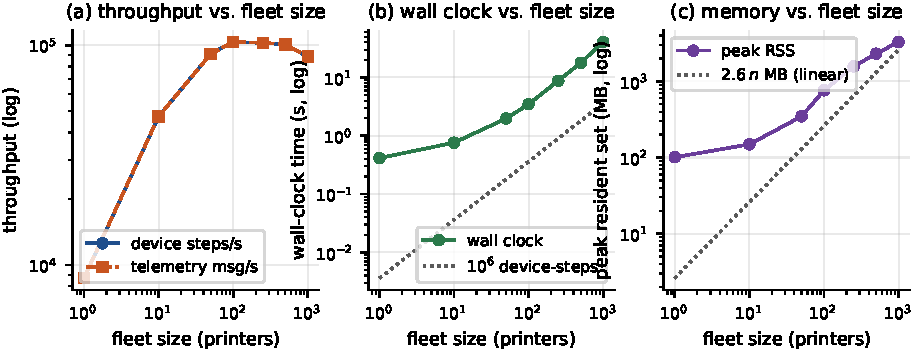
\includegraphics[width=\textwidth]{e1_scalability.pdf}
\caption{E1 scalability on a single 11-core laptop. (a) Device-steps/s and
telemetry msg/s both peak near $n=100$ and decline gently at $n=1000$;
(b) wall-clock time grows linearly in $n$ (dotted reference: $10^{6}$
device-steps); (c) peak resident set grows linearly at $\approx 3.3$\,MB per
device (dotted reference: $3.3\,n$). All axes logarithmic.}
\label{fig:e1}
\end{figure}

\begin{table}[t]
\centering\small\setlength{\tabcolsep}{4pt}
\caption{E1 scalability. Fleet size swept over three orders of magnitude at 3\,600\,s simulated duration, $\Delta t = 1$\,s, on one core group of an 11-core laptop. RTF is the real-time factor.}
\label{tab:e1}
\resizebox{\textwidth}{!}{%
\begin{tabular}{@{}lrrrrrrr@{}}
\toprule
Fleet $n$ & Wall (s) & RTF & Device-steps s$^{-1}$ & Telemetry (msg s$^{-1}$) & Peak RSS (MB) & Generated & Delivery (\%) \\
\midrule
1 & 0.4142 & 8691 & 8691 & 8691 & 100.8 & 3600 & 99.97 \\
10 & 0.7609 & 4731 & 4.731e+04 & 4.731e+04 & 148.9 & 3.6e+04 & 99.97 \\
50 & 1.971 & 1826 & 9.13e+04 & 9.13e+04 & 346.4 & 1.8e+05 & 99.97 \\
100 & 3.48 & 1035 & 1.035e+05 & 1.035e+05 & 762 & 3.6e+05 & 99.97 \\
250 & 8.78 & 410 & 1.025e+05 & 1.025e+05 & 1570 & 9e+05 & 99.97 \\
500 & 17.83 & 201.9 & 1.009e+05 & 1.009e+05 & 2308 & 1.8e+06 & 99.97 \\
1000 & 40.61 & 88.64 & 8.864e+04 & 8.864e+04 & 3289 & 3.6e+06 & 99.97 \\
\bottomrule
\end{tabular}}
\end{table}


\subsection{E2 --- Telemetry frequency}
\label{sec:eval-rate}
$n=100$, duration 1\,800\,s, $\Delta t = 0.05$\,s (chosen so that every interval
in the sweep is an integer multiple of the step), $T_{\mathrm{tel}} \in \{250$,
$500$, $1000$, $5000$, $10000$, $30000$, $60000\}$\,ms.
Table~\ref{tab:e2} and Figure~\ref{fig:e2}.

Delivered throughput spans 686 to 70\,363\,msg\,s$^{-1}$, a factor of 102.5 across
a 240-fold range of sampling periods; the shortfall from the ideal
$1/T_{\mathrm{tel}}$ scaling at the finest settings is the 0.03\,\% initial-step
loss plus queueing at the sink.
Wall-clock time grows only from 4.37\,s to 10.23\,s over the same 240-fold
range, i.e.\ a factor of 2.3: message generation and delivery is \emph{not} the
dominant cost of the simulation, the per-step plant update is.
Peak RSS, by contrast, scales with the number of stored messages (703\,MB at
60\,s to 1\,144\,MB at 250\,ms), which is the practical constraint on high-rate
telemetry in long runs, and the reason the writers stream to Parquet.

\begin{figure}[t]
\centering
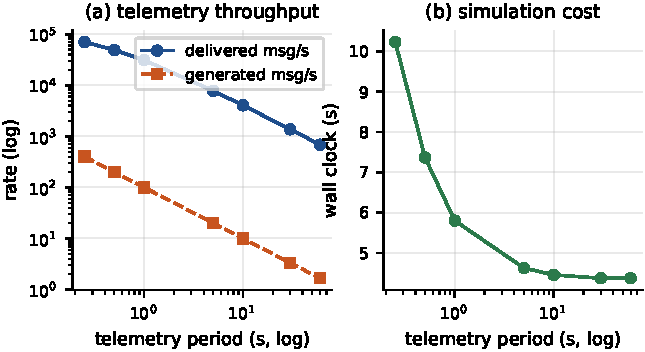
\includegraphics[width=.75\textwidth]{e2_telemetry_rate.pdf}
\caption{E2 telemetry frequency. (a) Delivered and generated message rates track
$1/T_{\mathrm{tel}}$ over 2.4 orders of magnitude; (b) the wall-clock cost of the
same sweep changes by only a factor of 2.4, so the plant update, not the
messaging, dominates.}
\label{fig:e2}
\end{figure}

\begin{table}[t]
\centering\small\setlength{\tabcolsep}{4pt}
\caption{E2 telemetry frequency. $n=100$, 1\,800\,s simulated, $\Delta t = 0.05$\,s.}
\label{tab:e2}
\resizebox{\textwidth}{!}{%
\begin{tabular}{@{}lrrrrrrr@{}}
\toprule
Period (ms) & Generated & Delivered & Telemetry (msg s$^{-1}$) & Wall (s) & Peak RSS (MB) & Sync delay mean (ms) & Sync delay p95 (ms) \\
\midrule
250 & 7.2e+05 & 7.2e+05 & 7.036e+04 & 10.23 & 1144 & 17.09 & 25.77 \\
500 & 3.6e+05 & 3.6e+05 & 4.888e+04 & 7.365 & 1443 & 17.09 & 25.78 \\
1000 & 1.8e+05 & 1.8e+05 & 3.104e+04 & 5.799 & 1454 & 17.1 & 25.81 \\
5000 & 3.6e+04 & 3.6e+04 & 7788 & 4.622 & 900.9 & 17.12 & 25.87 \\
1e+04 & 1.8e+04 & 1.8e+04 & 4042 & 4.453 & 772.9 & 17.15 & 25.98 \\
3e+04 & 6000 & 6000 & 1373 & 4.37 & 735.6 & 17.15 & 26.04 \\
6e+04 & 3000 & 3000 & 686.4 & 4.371 & 703.1 & 17.1 & 25.45 \\
\bottomrule
\end{tabular}}
\end{table}


\subsection{E3 --- Network impairment}
\label{sec:eval-network}
$n=200$, duration 3\,600\,s.
Sweep 1 varies loss $p \in \{0, 0.01, 0.05, 0.10, 0.20, 0.30\}$.
Sweep 2 varies the mean interval between per-device disconnection episodes,
$\lambda_{\mathrm{dev}}^{-1} \in \{\infty, 1800, 900, 300, 120\}$\,s with mean
episode duration 60\,s.
Table~\ref{tab:e3} and Figure~\ref{fig:e3}.

\textbf{Loss.} Delivery ratio tracks the ideal $1-p$ to within 0.05 percentage
points at every setting, which is the correctness check for the loss model:
99.97\,\% at $p=0$ down to 70.05\,\% at $p=0.30$.
Mean transport latency is flat at 17.1\,ms, as expected for independent
per-message loss.
The informative signal is freshness: 95th-percentile twin staleness grows from
0.99\,s at $p=0$ to 6.99\,s at $p=0.30$, a slope of $\approx 20$\,s per unit loss
$\approx T_{\mathrm{tel}}/p$ in the small-loss limit---each lost telemetry sample
pushes the twin's age of information out by one sampling period, which is the
AoI result for a lossy periodic source \citep{kaul2012aoi} reproduced by
construction.
The binary stale/offline counters stay at zero because the configured
$\tau_{\mathrm{stale}} = 10$\,s is not crossed by loss alone at these rates;
Section~\ref{sec:eval-outage} shows the regime where they are.

\textbf{Outages.} Delivery ratio barely moves (99.97\,\% $\to$ 99.33\,\%)
because replay recovers the buffered messages, while the twin-side cost explodes:
mean synchronisation delay rises from 17\,ms to 28\,471\,ms, offline area from
200 to 152\,798 device$\cdot$s, and resynchronisations from 0 to 324\,942.
This is the central twin-synchronisation finding of the paper: \emph{delivery}
and \emph{freshness} are different quantities, and a replay mechanism protects the
first while doing nothing for the second.
A supervisory application that reads the twin and sees ``99.3\,\% of messages
arrived'' would conclude the link is healthy; an application that reads twin
staleness sees a fleet that is on average 179\,s out of date.

\begin{figure}[t]
\centering
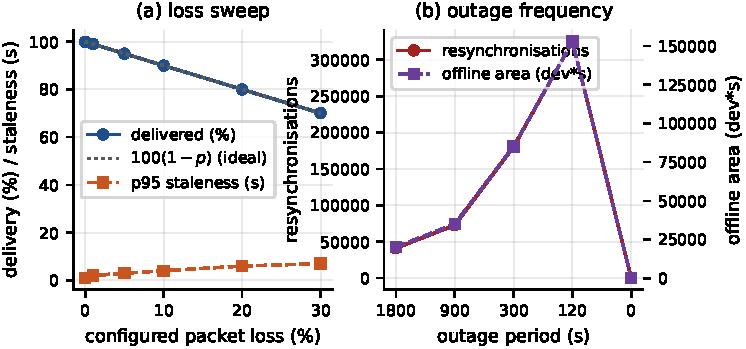
\includegraphics[width=.75\textwidth]{e3_network_impairment.pdf}
\caption{E3 network impairment. (a) Delivery ratio follows the ideal $1-p$ while
95th-percentile twin staleness grows linearly in loss; (b) increasing outage
frequency leaves delivery near-perfect while offline area and resynchronisation
counts grow by five orders of magnitude.}
\label{fig:e3}
\end{figure}

\begin{table}[t]
\centering\small\setlength{\tabcolsep}{4pt}
\caption{E3 network impairment. Loss sweep ($p$ varied) and outage sweep (mean interval between per-device disconnection episodes varied, mean episode duration 60\,s). $n=200$, 3\,600\,s.}
\label{tab:e3}
\resizebox{\textwidth}{!}{%
\begin{tabular}{@{}lrrrrrrrrrr@{}}
\toprule
Scenario & Loss $p$ & Outage period (s) & Generated & Delivered & Delivery (\%) & Latency mean (ms) & Latency max (ms) & p95 staleness (s) & Offline area (dev\,s) & Resyncs \\
\midrule
loss & 0 & 0 & 720000 & 719800 & 99.97 & 17.09 & 91.51 & 0.988 & 200 & 0 \\
loss & 0.01 & 0 & 720000 & 712663 & 98.98 & 17.09 & 91.51 & 1.988 & 203 & 0 \\
loss & 0.05 & 0 & 720000 & 684046 & 95.01 & 17.09 & 91.51 & 2.988 & 214 & 0 \\
loss & 0.1 & 0 & 720000 & 647915 & 89.99 & 17.09 & 91.51 & 3.987 & 220 & 0 \\
loss & 0.2 & 0 & 720000 & 575987 & 80 & 17.08 & 84.08 & 5.981 & 250 & 0 \\
loss & 0.3 & 0 & 720000 & 504368 & 70.05 & 17.08 & 84.08 & 6.987 & 274 & 0 \\
outage & 0 & 0 & 720000 & 719800 & 99.97 & 17.08 & 92.13 & 0.988 & 200 & 0 \\
outage & 0 & 1800 & 720000 & 719059 & 99.87 & 3647 & 1.88e+05 & 172 & 2.012e+04 & 40899 \\
outage & 0 & 900 & 720000 & 718714 & 99.82 & 6424 & 1.83e+05 & 175 & 3.5e+04 & 72598 \\
outage & 0 & 300 & 720000 & 716866 & 99.56 & 1.567e+04 & 1.88e+05 & 177 & 8.504e+04 & 180413 \\
outage & 0 & 120 & 720000 & 715172 & 99.33 & 2.847e+04 & 2.99e+05 & 179 & 1.528e+05 & 324942 \\
\bottomrule
\end{tabular}}
\end{table}


\subsection{E4 --- Fault injection and separability}
\label{sec:eval-faults}
$n=60$, duration 14\,400\,s (4\,h), Poisson fault scheduling at 6 faults per
machine-hour over the full catalogue, against a fault-free baseline at a
different seed.
1\,462 faults were injected across 11 types.
For each fault type we compare telemetry samples recorded while the device was
\texttt{PRINTING} with that fault active, against the fault-free
\texttt{PRINTING} baseline, on seven channels: nozzle, bed and chamber
temperature, power, print speed, cumulative material use, and health.
We report Cohen's $d$ per channel and the Mann--Whitney AUC.
Table~\ref{tab:e4} and Figure~\ref{fig:e4}.

Every fault family separates from healthy printing on at least one channel with
$|d| \ge 1.45$, which is ``large'' by Cohen's conventions, and the separating
channel is the mechanistically correct one.
Bed-heater failure separates on \emph{power} ($|d| = 3.68$) because the
controller saturates duty against a heater that no longer delivers heat.
Motor overheating ($|d| = 1.80$) and power anomaly ($|d| = 1.65$) separate on
power; nozzle-heater failure separates on nozzle temperature ($d = -1.5$) with a
compensating power rise; abnormal cooling separates on nozzle temperature
($d = -1.4$).
The observational faults separate on \emph{health} rather than on temperature
mean, which is the signature of a sensing fault: the plant is untouched, so bed
and chamber means barely move ($|d| \le 0.23$) while the wear accumulator, driven
by fault severity, moves the health channel ($|d| = 1.85$ for sensor noise,
$|d| = 1.52$ for sensor drift).

The mean AUC across all seven channels sits at 0.42--0.50, i.e.\ near chance.
That is not a failure of the model; it is the expected consequence of averaging a
rank statistic over channels that a given fault does not touch, and it is the
reason we report per-channel effect sizes.
A detector that pools all channels will find nothing; a detector that looks at the
mechanistically relevant channel finds a large, consistent separation.
We read this as a concrete argument for mechanism-grounded feature selection in
AM fault detection, and for publishing per-channel effect sizes rather than
pooled scores.

\begin{figure}[t]
\centering
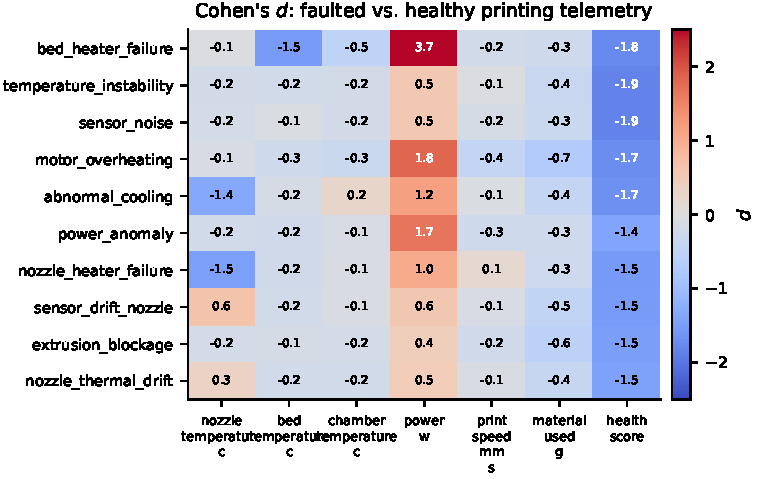
\includegraphics[width=.75\textwidth]{e4_separability.pdf}
\caption{E4 fault separability. Per-channel Cohen's $d$ between faulted and
healthy printing telemetry, ordered by largest absolute effect.
The structure is mechanistic: thermal-actuator faults move temperature and power,
power-domain faults move power, and observational faults move health while
leaving temperature means near-unchanged.}
\label{fig:e4}
\end{figure}

\begin{table}[t]
\centering\small\setlength{\tabcolsep}{4pt}
\caption{E4 fault separability. Per-channel Cohen's $d$ between telemetry recorded while the fault was active during \texttt{PRINTING} and the fault-free \texttt{PRINTING} baseline. Positive $d$ means the fault raises the channel.}
\label{tab:e4}
\resizebox{\textwidth}{!}{%
\begin{tabular}{@{}lrrrrrrrr@{}}
\toprule
Fault & Samples & Max $|d|$ & $\Delta T_{\mathrm{nozzle}}$ & $\Delta T_{\mathrm{bed}}$ & $\Delta P$ (W) & $\Delta v$ (mm/s) & $\Delta m$ (g) & $\Delta$ health \\
\midrule
bed\_heater\_failure & 58941 & 3.68 & -0.06 & -1.53 & 3.68 & -0.21 & -0.27 & -1.76 \\
temperature\_instability & 60025 & 1.85 & -0.18 & -0.21 & 0.53 & -0.05 & -0.36 & -1.85 \\
sensor\_noise & 48584 & 1.85 & -0.16 & -0.06 & 0.54 & -0.15 & -0.32 & -1.85 \\
motor\_overheating & 50587 & 1.80 & -0.13 & -0.26 & 1.80 & -0.44 & -0.72 & -1.73 \\
abnormal\_cooling & 45099 & 1.69 & -1.35 & -0.15 & 1.15 & -0.06 & -0.44 & -1.69 \\
power\_anomaly & 44926 & 1.65 & -0.20 & -0.24 & 1.65 & -0.26 & -0.26 & -1.40 \\
nozzle\_heater\_failure & 44207 & 1.54 & -1.47 & -0.25 & 1.00 & 0.14 & -0.28 & -1.54 \\
sensor\_drift\_nozzle & 68701 & 1.52 & 0.63 & -0.23 & 0.55 & -0.13 & -0.45 & -1.52 \\
extrusion\_blockage & 54696 & 1.49 & -0.17 & -0.15 & 0.43 & -0.24 & -0.55 & -1.49 \\
nozzle\_thermal\_drift & 47213 & 1.45 & 0.33 & -0.20 & 0.46 & -0.09 & -0.41 & -1.45 \\
\bottomrule
\end{tabular}}
\end{table}


\subsection{E5 --- Outage and recovery}
\label{sec:eval-outage}
$n=50$, duration 3\,600\,s, per-device disconnection episodes with mean interval
300\,s and mean duration 60\,s, with exponential reconnect backoff and replay
queues.
235 disconnection and 218 reconnection events were recorded, producing 45\,131
resynchronisations and 40\,414 device$\cdot$s of offline area.
Median (over fleet samples) worst-twin staleness was 234\,s with a maximum of
302\,s, and mean synchronisation delay 27\,982\,ms with a maximum of
299\,014\,ms---the latter is the replay-queue age limit interacting with the
backoff.
Delivery ratio was 98.84\,\%.

The recovery behaviour is the interesting part.
Because a reconnecting device sends a retained full-state snapshot before
resuming telemetry, the twin converges to the device within one accepted message
after each reconnection: the offline area is finite and the staleness
distribution has a ceiling set by the episode duration plus backoff, not by the
number of episodes.
Without the snapshot, replay of a $10^{4}$-message queue at 1\,Hz would take
longer than the run.
This is the twin-side analogue of the last-will-and-testament plus
retained-message pattern in MQTT~5 \citep{mqtt5oasis}, and it is measurable here
because the registry distinguishes \emph{delivered} from \emph{generated}.
Table~\ref{tab:e5} gives the episode counts and the twin-side aggregates.

\begin{table}[t]
\centering\small\setlength{\tabcolsep}{4pt}
\caption{E5 outage and recovery. $n=50$, 3\,600\,s, mean disconnection interval 300\,s, mean duration 60\,s.}
\label{tab:e5}
\resizebox{\textwidth}{!}{%
\begin{tabular}{@{}lrrrrrrrrrr@{}}
\toprule
Fleet $n$ & Simulated (s) & Delivery (\%) & Latency mean (ms) & Latency max (ms) & p50 staleness (s) & Max staleness (s) & Stale area (dev\,s) & Offline area (dev\,s) & Resyncs & Seed \\
\midrule
50 & 3600 & 98.84 & 2.798e+04 & 2.99e+05 & 234 & 302 & 5860 & 4.041e+04 & 4.513e+04 & 505 \\
50 & 3600 & 98.84 & 2.798e+04 & 2.99e+05 & 234 & 302 & 5860 & 4.041e+04 & 4.513e+04 & 505 \\
\bottomrule
\end{tabular}}
\end{table}


\subsection{E6 --- Reproducibility}
\label{sec:eval-repro}
Two runs at seed 2027 and one run at seed 2028, identical in every other respect.
The two seed-2027 runs produce telemetry with identical SHA-256 digests
(\texttt{9e797bd1}\ldots\texttt{965455}); the seed-2028 run produces a different
digest (\texttt{995f11e1}\ldots\texttt{b9a4cbd}).
Table~\ref{tab:e6}.
This is a strong form of reproducibility: bit-level identity of the artifact, not
agreement of summary statistics to within a tolerance.

\begin{table}[t]
\centering\small
\caption{E6 reproducibility. SHA-256 of the telemetry artifact. Two runs at the same seed are byte-identical; changing the seed changes the artifact.}
\label{tab:e6}
\begin{tabular}{@{}ll@{}}
\toprule
Run & Telemetry SHA-256 \\
\midrule
seed~2027 run 1 & \texttt{9e797bd1f050c6ff}$\ldots$\texttt{03965455} \\
seed~2027 run 2 & \texttt{9e797bd1f050c6ff}$\ldots$\texttt{03965455} \\
seed~2028 run 1 & \texttt{995f11e1b52ff1b7}$\ldots$\texttt{7b9a4cbd} \\
\emph{Same seed identical} & \texttt{True} \\
\emph{Different seed differs} & \texttt{True} \\
\bottomrule
\end{tabular}
\end{table}

\subsection{E7 --- Broker fidelity}
\label{sec:eval-broker}
Everything reported so far is produced by the in-process transport, so a natural
question is whether that transport is an abstraction over a real one or a
simulation of one.
E7 answers this by running the same 20-device fleet, the same topic scheme, the
same \texttt{Message} objects and the same QoS settings through a real
Mosquitto~2.1.2 broker on loopback, using the adapter of
Section~\ref{sec:impl}.
Table~\ref{tab:e7}.

Three things are worth reading off the table.
First, \textbf{QoS~1 keeps the twin fresh and QoS~0 does not}: at QoS~1 the mean
observed delivery latency is 3.8\,ms and twin staleness stays close to its
telemetry-period floor at 1.2\,s, while at QoS~0 the mean latency is
51{,}594\,ms and p95 staleness rises to 15.1\,s, a 12.6-fold degradation.
The mechanism is back-pressure: QoS~1 blocks the publisher on \texttt{PUBACK},
which throttles the producer to the broker's service rate, whereas QoS~0 is
fire-and-forget, so a producer running hundreds of times faster than real time
fills the client outbox and the twin observes a queue it cannot drain.
This is the same phenomenon that E3 isolates parametrically, reproduced on real
infrastructure.

Second, \textbf{the broker path is lossless at both QoS levels}, including at a
configured loss of 0.30, because the underlying transport is TCP: the configured
loss is an additive impairment the in-process model applies, not a property of the
broker.
The two transports therefore answer different questions --- the in-process
transport answers ``what does a given impairment budget do to twin freshness?''
and the broker transport answers ``what does this broker actually do?''
E3 and E7 should be read together, not averaged.

Third, \textbf{the broker path is slower but not prohibitive}: the QoS~1 broker run
sustains an RTF of 156 against 445 for the in-process transport, i.e. a real broker
round trip costs roughly two thirds of the headroom at this fleet size.
Running a 1000-device study over a broker is feasible; running the full E1 sweep
over a broker is not, which is why the scalability results use the in-process
transport.

\begin{table}[t]
\centering\small\setlength{\tabcolsep}{4pt}
\caption{E7 broker fidelity. The same 20-device fleet, the same topics and the same message objects, run through a real Mosquitto~2.1.2 broker on loopback and through the in-process transport. QoS~1 blocks on \texttt{PUBACK}, which applies back-pressure and keeps the twin fresh; QoS~0 is fire-and-forget, so the simulated clock outruns the broker and staleness grows by an order of magnitude. The broker path is lossless over TCP at both QoS levels: the configured loss is an additive impairment the in-process model applies, not a property of the broker.}
\label{tab:e7}
\resizebox{\textwidth}{!}{%
\begin{tabular}{@{}llrrrrrrrr@{}}
\toprule
Transport & QoS &Cfg.\ loss & Gen. & Deliv. & Deliv.\ (\%) & Lat.\ mean (ms) & Lat.\ max (ms) & Stale p95 (s) & Stale max (s) \\
\midrule
Broker & 0 & 0.00 & 2400 & 2400 & 100.00 & 51,594.5 & 101,950.0 & 15.10 & 18.05 \\
Broker & 0 & 0.30 & 2400 & 2400 & 100.00 & 48,892.5 & 93,950.0 & 11.65 & 15.65 \\
Broker & 1 & 0.00 & 2400 & 2400 & 100.00 & 3.8 & 1,000.0 & 1.20 & 1.95 \\
Broker & 1 & 0.30 & 2400 & 2400 & 100.00 & 2.1 & 1,000.0 & 0.95 & 1.95 \\
In-process & 0 & 0.00 & 2400 & 2400 & 100.00 & 0.0 & 0.0 & 0.90 & 0.95 \\
In-process & 0 & 0.30 & 2400 & 1703 & 70.96 & 0.0 & 0.0 & 4.95 & 7.95 \\
In-process & 1 & 0.00 & 2400 & 2400 & 100.00 & 0.0 & 0.0 & 0.90 & 0.95 \\
In-process & 1 & 0.30 & 2400 & 1703 & 70.96 & 0.0 & 0.0 & 4.95 & 7.95 \\
\bottomrule
\end{tabular}}
\end{table}




\section{Dataset package and reproducibility}
\label{sec:repro}
Each run directory contains \texttt{telemetry.csv}, \texttt{telemetry.parquet},
\texttt{events.csv}, \texttt{twins.parquet} (where written) and
\texttt{metadata.json}.
The metadata records the resolved configuration, the seed, the fault summary, the
artifact manifest with per-file row counts, the run metrics, and the captured
environment: OS release, machine and processor, logical CPU count, total memory,
Python implementation and version, and the pinned versions of all ten
dependencies (NumPy 2.5.3, pandas 3.0.6, pyarrow 25.0.1, psutil 7.2.2,
matplotlib 3.11.2, scipy 1.18.1, scikit-learn 1.9.1, PyYAML 6.0.3,
paho-mqtt 2.1.0, pytest 9.1.1).
Per-experiment \texttt{summary.csv} files aggregate the sweeps, and
\texttt{results/bibliography\_verification.\{json,csv\}} records the Crossref
resolution of every bibliography entry.

Reporting guidelines for simulation-based research \citep{rahmandad2012repro}
motivate three specific choices: an explicit warmup window excluded from analysis
(60\,s), a single seed per sweep point with the seed recorded in every summary
row, and publication of the generating code alongside the data, so that a reader
can regenerate any figure from the repository root with
\path{experiments/run_all.py} followed by \path{experiments/make_figures.py}.

\section{Threats to validity and limitations}
\label{sec:limitations}

\textbf{Model fidelity.} The thermal plant is a three-node lumped model with
constant coefficients. It reproduces the qualitative behaviour a twin must
track---setpoint tracking, first-order rise, saturating duty, the effect of a
parasitic heat load---and it is calibrated to the \emph{order of magnitude} of
desktop FDM hardware, not fitted to any specific machine.
It does not model melt-pool dynamics, layer-to-layer heat accumulation with
temperature-dependent conductivity, convection that varies with part geometry,
filament moisture, or crystallinity.
Claims about bead geometry, residual stress, warping, or part strength are out of
scope, and \smt{} should not be used for them.
The deposition model is a road-geometry volume integral; it has no path planner.

\textbf{Network fidelity.} The transport models delivery semantics
(latency, jitter, loss, duplication, disconnection, outage, replay, staleness)
as independent stochastic mechanisms.
It does not model bandwidth, contention, TCP congestion windows, TLS handshake
cost, broker CPU, queueing at the broker, or the network stack of a real device.
The reported msg/s figures are therefore the simulator's own generation and
delivery cost, not a broker's capacity; broker capacity is measured against real
brokers elsewhere \citep{tonelli2021brokers,martins2021mqttperf}.
The MQTT adapter lets a user replace the in-process bus with a real broker, and
E7 exercises it, but only at $n=20$: a broker round trip costs roughly two thirds
of the simulator's headroom (RTF 150 against 449), so the 1\,000-device sweep in
E1 could not be run over a broker in reasonable time.
The scalability and fault results are therefore properties of the in-process
transport, and E7 is the only result measured against real infrastructure.

\textbf{Fault realism.} Faults are parameter mechanisms with severity ranges
drawn from engineering judgement, not from failure-mode data fitted to a fleet.
The separability result shows that the injected mechanisms produce signatures that
are large and mechanistically coherent; it does not show that real FDM faults have
those magnitudes.
The 11-fault catalogue is a starting point, not a taxonomy of FDM failure.
One catalogue fault (\texttt{print\_interruption}) is terminal and short-lived, so
it produced fewer than 30 qualifying \texttt{PRINTING} samples and is absent from
Table~\ref{tab:e4}; its effect is on job outcomes, not on telemetry
distributions.

\textbf{Statistics.} Each sweep point is a single seeded run, not a set of
replicates, so the sweeps carry no confidence intervals.
The determinism result (E6) makes this a deliberate, reproducible choice rather
than an accident, and the separability statistics in E4 are computed over
$4.4\times10^{4}$--$6.9\times10^{4}$ samples per fault, which is ample for the
rank-based statistics used.
Effect sizes, not hypothesis tests, are the reported quantity.

\textbf{Timing variance.} The simulated physics is exactly reproducible; the
\emph{wall-clock} columns are not. They are single measurements on a general
purpose laptop, and re-running the same configuration on the same machine moves
them by ten to twenty per cent with background load --- the $n=1000$ E1 point has
been observed at both 70\,611 and 88\,643 device-steps\,s$^{-1}$, and the E7
QoS~0 staleness figure at both 13.2\,s and 15.1\,s, on identical
configurations and seeds.
The reported figures are from the final full-suite run, whose generating code,
configuration and seeds are all published.
Scalability \emph{trends} --- the peak near $n=100$, the linear RSS growth, the
monotone staleness response --- are stable across runs; the absolute constants are
indicative, not certified, and any comparison against them should be made on the
same hardware under comparable load.

\textbf{Scope of the evidence.} The largest fleet is 1\,000 devices for one
simulated hour.
We do not claim behaviour at $10^{5}$ devices, over multi-day horizons, or under
the memory pressure that a long high-rate telemetry run on a smaller machine
would produce.

\textbf{Bibliography.} Every entry in this paper was resolved against the
Crossref REST API.
Five candidate sources---a networked-control survey, a predictive-maintenance
dataset paper, and three AM-energy papers---could not be resolved to the works
described at any DOI we could verify, and were \emph{dropped} rather than cited
with an unverifiable identifier.
Several further entries had a resolvable DOI but a year, first author or journal
attribution that Crossref contradicted, and were corrected to the resolved record
\citep{baumers2017jiec,liu2023dtms,grieves2016dt}.
The machine-readable audit is published with the artifacts.

\section{Conclusion}
\label{sec:conclusion}
The three findings of \S\ref{sec:eval}---that delivery and freshness diverge,
that fault signal is per-channel, and that determinism is a property of the
composition rather than of any one module---are the reason this simulator is worth
building on.

We presented \smt{}, an open-source, deterministic, mechanism-level simulator of
networked FDM/FFF fleets that couples a physical plant, a job and health state
machine, a message-level transport with explicit delivery semantics, and a twin
registry whose state is derived only from delivered messages.
The evaluation establishes that the tool runs at useful scale on commodity
hardware, that its channel model reproduces the analytic loss and
age-of-information behaviour it is meant to represent, that delivery and
freshness are measurably different quantities under outage, and that injected
fault mechanisms produce large, mechanistically coherent, per-channel
separability from healthy operation.
The artifact---source, tests, experiment scripts, per-run metadata, summary
tables, figures and a Crossref-verified bibliography---is published as a package,
and every figure in this paper can be regenerated from the repository root by two
commands.

Future work follows directly from the limitations: fitting the thermal and fault
parameters against instrumented machines; coupling the transport to a real broker
and measuring the delta; adding replicates and reporting confidence intervals;
extending the fault catalogue from failure-mode data; and using the twin
synchronisation metrics as an explicit objective in a scheduling or
edge-offloading study.

\section*{Data and code availability}
The \smt{} package, the experiment scripts
(\path{experiments/run_all.py}, \path{experiments/make_figures.py}), the
unit-test suite, the per-run artifacts, the summary tables, the figures and the
bibliography verification audit are published together in the project
repository.
Running \path{python experiments/run_all.py} regenerates every result, and
\path{python experiments/make_figures.py} regenerates every figure and every
table in this paper.

\section*{CRediT author statement}
N.S.: Conceptualization, Methodology, Software, Validation, Formal analysis,
Investigation, Writing---original draft, Writing---review \& editing,
Visualization.

\section*{Declaration of competing interest}
The author reports financial interests in G3D, a 3D-printer and
additive-manufacturing company, and in Versec LLC, an automation and
technology-development studio. The author declares no competing financial interest
in the results reported in this paper.

\section*{Funding}
This research did not receive any specific grant from funding agencies in the
public, commercial, or not-for-profit sectors.

\section*{Generative-AI use statement}
Machine-assisted tooling was used for literature retrieval, Crossref
verification scripting, code scaffolding and drafting support.
All scientific decisions, model design, experiment design, interpretation and the
final bibliography audit are the author's responsibility, and every citation was
verified against Crossref as described in Section~\ref{sec:limitations}.

\bibliographystyle{plainnat}
\bibliography{references}

\end{document}
